% Power BI Automated Validation Framework -- Sequence diagram
%
% Scenario: "Dispute status by dispute code chart reconciles against Snowflake"
% (features/powerbi_validation.feature), traced against the actual
% implementation in features/steps/test_powerbi_validation_steps.py
% (_load_grouped_mapping / _reconcile_grouped / _assert_grouped_reconciliation).
%
% Compile with: pdflatex docs/sequence_grouped_reconciliation.tex (or Overleaf)
% Not compiled/verified locally -- no LaTeX install on the machine this was
% authored on. Hand-rolled in plain TikZ (no tikz-uml/pgf-umlsd dependency)
% specifically so it doesn't depend on a UML package that may or may not be
% present in whatever distribution compiles this -- only core TikZ libraries
% that ship with every install. Absolute `at (x,y)` coordinates throughout,
% same reasoning as docs/architecture_wireframe.tex: minimizes the kind of
% compounding alignment risk that can't be caught without a compiler.
%
% Deliberately omits UML activation bars (the thin rectangles marking when a
% lifeline is "busy") -- they require precise per-actor start/end tracking
% that adds real collision risk without a compiler to check it, and the call
% order + labels already carry the information this diagram needs to convey.

\documentclass[tikz,border=14pt]{standalone}
\usepackage{tikz}
\usetikzlibrary{arrows.meta, fit, backgrounds}

\begin{document}
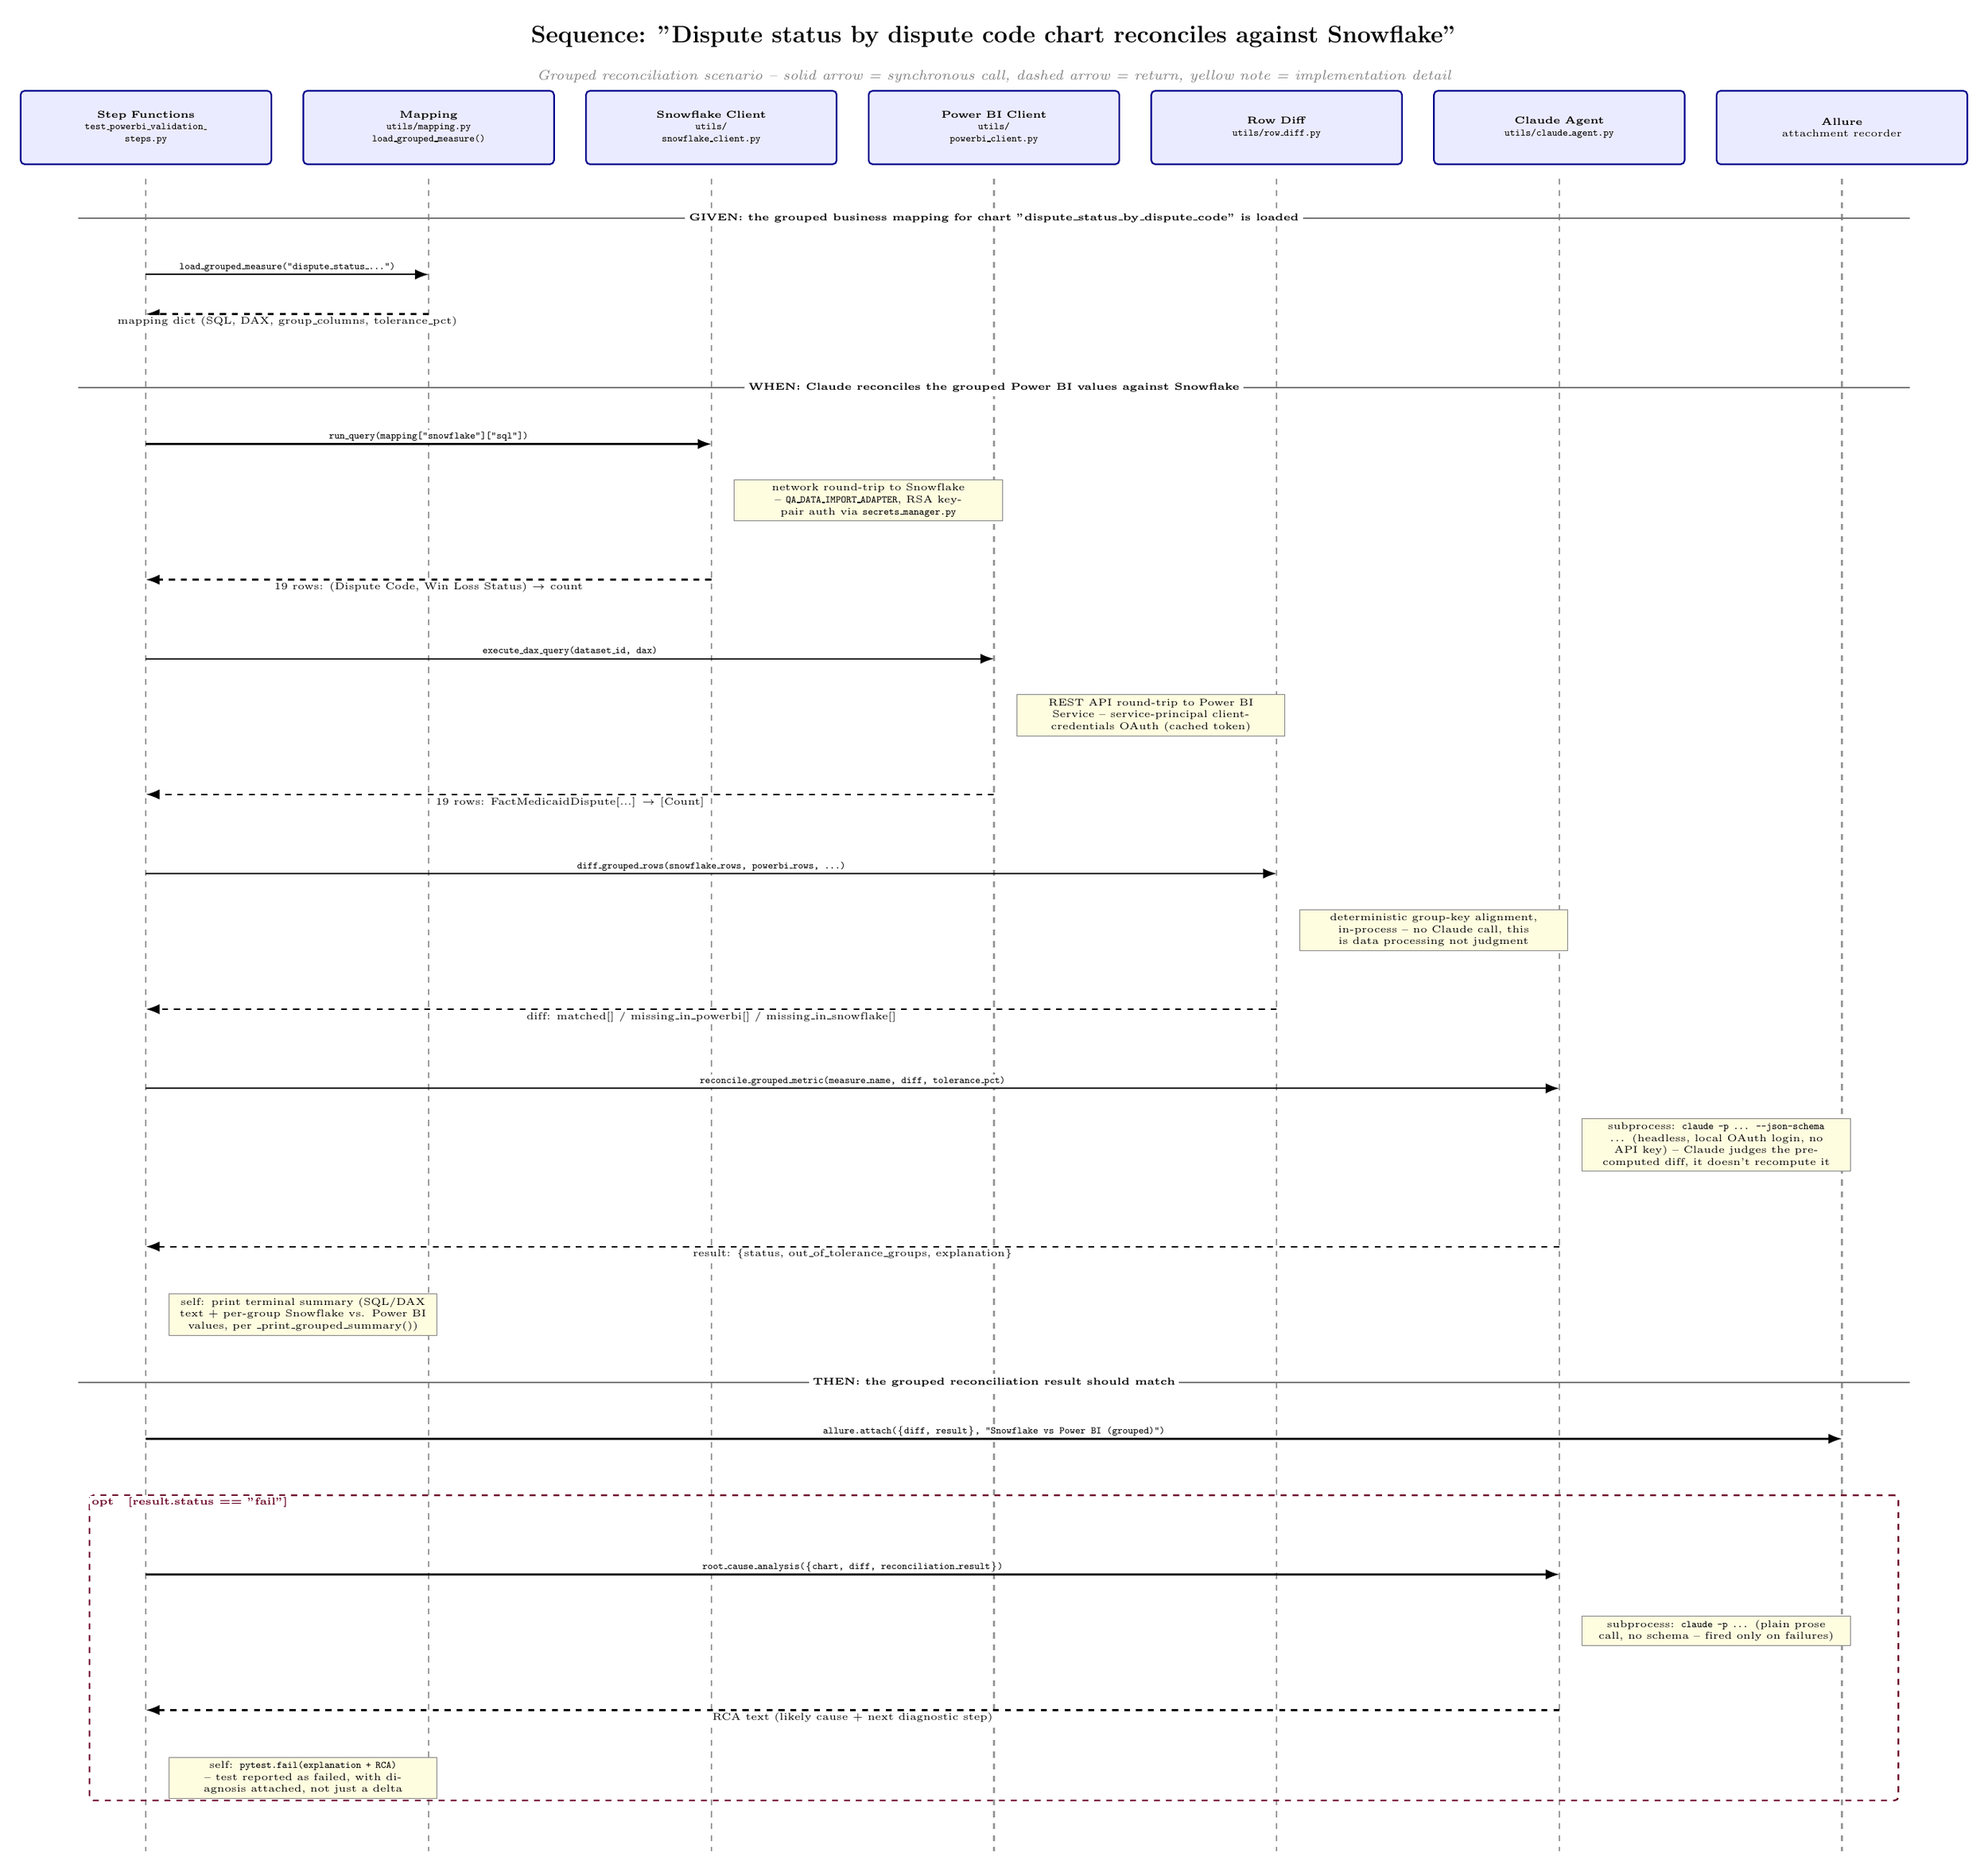
\begin{tikzpicture}[
  font=\sffamily,
  every node/.style={align=center},
  actorbox/.style={rectangle, rounded corners=2pt, draw=blue!55!black, thick,
    fill=blue!8, text width=4.2cm, minimum height=1.3cm, font=\tiny},
  lifeline/.style={draw=black!40, dashed, thick},
  syncmsg/.style={-{Latex[length=2.4mm]}, thick},
  retmsg/.style={-{Latex[length=2.4mm]}, thick, dashed},
  notebox/.style={rectangle, draw=black!50, fill=yellow!12, thin,
    text width=4.6cm, font=\tiny, inner sep=2pt},
  msglabel/.style={font=\tiny, fill=white, inner sep=1pt},
  divider/.style={draw=black!55, thick},
  dividerlabel/.style={font=\bfseries\tiny, fill=white, inner sep=2pt},
  optframe/.style={draw=purple!55!black, dashed, thick, rounded corners=2pt},
  optlabel/.style={font=\bfseries\tiny, text=purple!55!black, fill=white, inner sep=1pt}
]

% =====================================================================
% LAYOUT GRID (cm): 7 actor columns at x = 0,5,10,15,20,25,30
% Time flows downward (y decreasing). Header boxes at y=0; lifelines run
% from y=-0.9 to y=-30.5.
% =====================================================================

% Title
\node[font=\bfseries\large] at (15, 1.6)
  {Sequence: "Dispute status by dispute code chart reconciles against Snowflake"};
\node[font=\itshape\scriptsize, text=black!50] at (15, 0.9)
  {Grouped reconciliation scenario -- solid arrow = synchronous call,
   dashed arrow = return, yellow note = implementation detail};

% ---------------------------------------------------------------------
% Actor headers
% ---------------------------------------------------------------------
\node[actorbox] (a1) at (0, 0)
  {\textbf{Step Functions}\\\texttt{test\_powerbi\_validation\_}\\\texttt{steps.py}};
\node[actorbox] (a2) at (5, 0)
  {\textbf{Mapping}\\\texttt{utils/mapping.py}\\\texttt{load\_grouped\_measure()}};
\node[actorbox] (a3) at (10, 0)
  {\textbf{Snowflake Client}\\\texttt{utils/}\\\texttt{snowflake\_client.py}};
\node[actorbox] (a4) at (15, 0)
  {\textbf{Power BI Client}\\\texttt{utils/}\\\texttt{powerbi\_client.py}};
\node[actorbox] (a5) at (20, 0)
  {\textbf{Row Diff}\\\texttt{utils/row\_diff.py}};
\node[actorbox] (a6) at (25, 0)
  {\textbf{Claude Agent}\\\texttt{utils/claude\_agent.py}};
\node[actorbox] (a7) at (30, 0)
  {\textbf{Allure}\\attachment recorder};

% Lifelines
\foreach \x in {0,5,...,30} {
  \draw[lifeline] (\x, -0.9) -- (\x, -30.5);
}

% ---------------------------------------------------------------------
% GIVEN
% ---------------------------------------------------------------------
\draw[divider] (-1.2, -1.6) -- (31.2, -1.6);
\node[dividerlabel] at (15, -1.6)
  {GIVEN: the grouped business mapping for chart "dispute\_status\_by\_dispute\_code" is loaded};

\draw[syncmsg] (0,-2.6) -- (5,-2.6)
  node[midway, above, msglabel] {\texttt{load\_grouped\_measure("dispute\_status\_...")}};
\draw[retmsg] (5,-3.3) -- (0,-3.3)
  node[midway, below, msglabel] {mapping dict (SQL, DAX, group\_columns, tolerance\_pct)};

% ---------------------------------------------------------------------
% WHEN
% ---------------------------------------------------------------------
\draw[divider] (-1.2, -4.6) -- (31.2, -4.6);
\node[dividerlabel] at (15, -4.6)
  {WHEN: Claude reconciles the grouped Power BI values against Snowflake};

\draw[syncmsg] (0,-5.6) -- (10,-5.6)
  node[midway, above, msglabel] {\texttt{run\_query(mapping["snowflake"]["sql"])}};
\node[notebox, anchor=west] at (10.4,-6.6)
  {network round-trip to Snowflake -- \texttt{QA\_DATA\_IMPORT\_ADAPTER},
   RSA key-pair auth via \texttt{secrets\_manager.py}};
\draw[retmsg] (10,-8.0) -- (0,-8.0)
  node[midway, below, msglabel] {19 rows: (Dispute Code, Win Loss Status) $\to$ count};

\draw[syncmsg] (0,-9.4) -- (15,-9.4)
  node[midway, above, msglabel] {\texttt{execute\_dax\_query(dataset\_id, dax)}};
\node[notebox, anchor=west] at (15.4,-10.4)
  {REST API round-trip to Power BI Service -- service-principal
   client-credentials OAuth (cached token)};
\draw[retmsg] (15,-11.8) -- (0,-11.8)
  node[midway, below, msglabel] {19 rows: FactMedicaidDispute[...] $\to$ [Count]};

\draw[syncmsg] (0,-13.2) -- (20,-13.2)
  node[midway, above, msglabel] {\texttt{diff\_grouped\_rows(snowflake\_rows, powerbi\_rows, ...)}};
\node[notebox, anchor=west] at (20.4,-14.2)
  {deterministic group-key alignment, in-process --
   no Claude call, this is data processing not judgment};
\draw[retmsg] (20,-15.6) -- (0,-15.6)
  node[midway, below, msglabel] {diff: matched[] / missing\_in\_powerbi[] / missing\_in\_snowflake[]};

\draw[syncmsg] (0,-17.0) -- (25,-17.0)
  node[midway, above, msglabel] {\texttt{reconcile\_grouped\_metric(measure\_name, diff, tolerance\_pct)}};
\node[notebox, anchor=west] at (25.4,-18.0)
  {subprocess: \texttt{claude -p ... --json-schema ...} (headless,
   local OAuth login, no API key) -- Claude judges the precomputed
   diff, it doesn't recompute it};
\draw[retmsg] (25,-19.8) -- (0,-19.8)
  node[midway, below, msglabel] {result: \{status, out\_of\_tolerance\_groups, explanation\}};

\node[notebox, anchor=west] at (0.4,-21.0)
  {self: print terminal summary (SQL/DAX text + per-group Snowflake vs.
   Power BI values, per \_print\_grouped\_summary())};

% ---------------------------------------------------------------------
% THEN
% ---------------------------------------------------------------------
\draw[divider] (-1.2, -22.2) -- (31.2, -22.2);
\node[dividerlabel] at (15, -22.2)
  {THEN: the grouped reconciliation result should match};

\draw[syncmsg] (0,-23.2) -- (30,-23.2)
  node[midway, above, msglabel] {\texttt{allure.attach(\{diff, result\}, "Snowflake vs Power BI (grouped)")}};

% ---------------------------------------------------------------------
% opt [result.status == "fail"]
% ---------------------------------------------------------------------
\node[optframe, fit={(-1.0,-24.2) (31.0,-29.6)}, inner sep=0] (optbox) {};
\node[optlabel, anchor=north west] at (-1.0,-24.2)
  {opt \; [result.status == "fail"]};

\draw[syncmsg] (0,-25.6) -- (25,-25.6)
  node[midway, above, msglabel] {\texttt{root\_cause\_analysis(\{chart, diff, reconciliation\_result\})}};
\node[notebox, anchor=west] at (25.4,-26.6)
  {subprocess: \texttt{claude -p ...} (plain prose call, no schema --
   fired only on failures)};
\draw[retmsg] (25,-28.0) -- (0,-28.0)
  node[midway, below, msglabel] {RCA text (likely cause + next diagnostic step)};
\node[notebox, anchor=west] at (0.4,-29.2)
  {self: \texttt{pytest.fail(explanation + RCA)} -- test reported as
   failed, with diagnosis attached, not just a delta};

\end{tikzpicture}
\end{document}
